% 9 variables in here:
% h_1 = 11.0, h_2 = 12.0, h_3 = 9.0, ux_1 = 2.0, ux_2 = -3.0, ux_3 = 1.0, uy_1 = 3.0, uy_2 = 2.0, uy_3 = -3.0
\begin{figure}[h!]
\centering
  \quad \subfloat[Height vales are $h_1=12, h_3=9$, $h_1$ ranges from 8 to 12.] {
    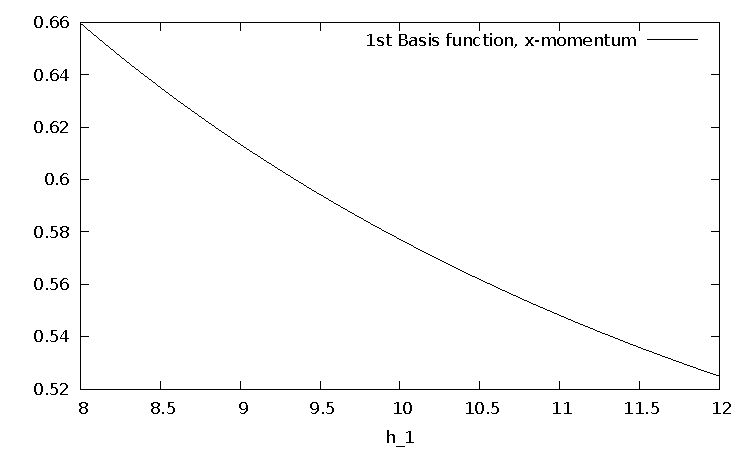
\includegraphics[scale=\zoomfactor]{{{magnitude_10_heights_momentums/y_12.0_9.0_2.0_-3.0_1.0_3.0_2.0_-3.0f00}}}
  }
  \hspace{.5cm}
  \quad \subfloat[Height vales are $h_1=12, h_3=9$, $h_1$ ranges from 8 to 12.] {
    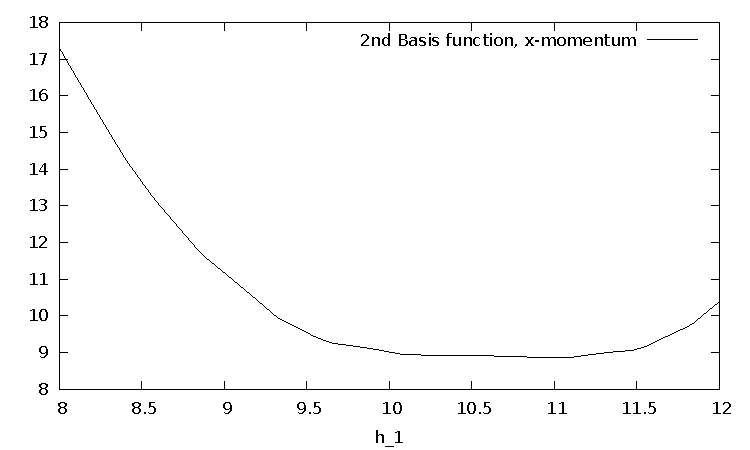
\includegraphics[scale=\zoomfactor]{{{magnitude_10_heights_momentums/y_12.0_9.0_2.0_-3.0_1.0_3.0_2.0_-3.0f02}}}
  }
  
  \quad \subfloat[Height values are $h_2=1002, h_3=999$, $h_1$ ranges from 998 to 1002.] {
    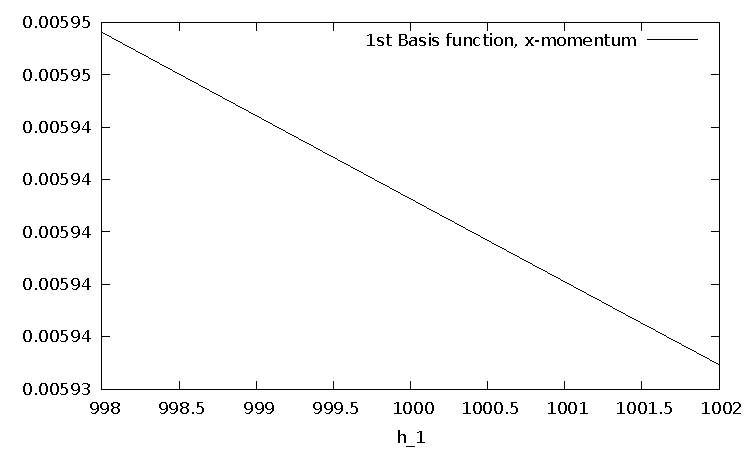
\includegraphics[scale=\zoomfactor]{{{magnitude_1000_heightsmomentums/y_1002.0_999.0_2.0_-3.0_1.0_3.0_2.0_-3.0f00}}}
  }
  \hspace{.5cm}
  \quad \subfloat[Height values are $h_2=1002, h_3=999$, $h_1$ ranges from 998 to 1002.] {
    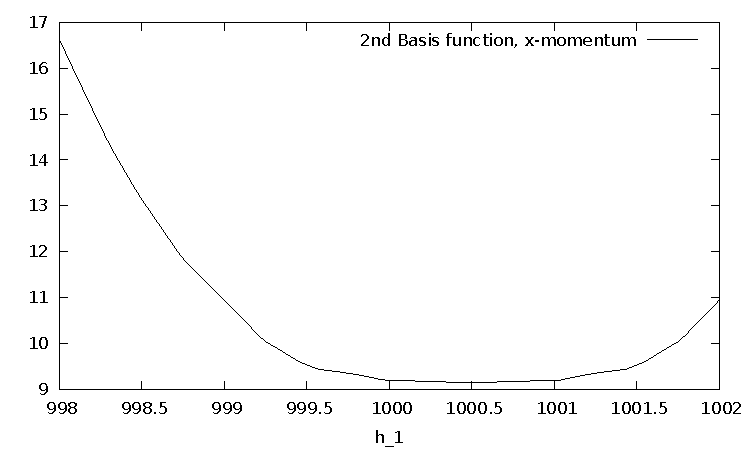
\includegraphics[scale=\zoomfactor]{{{magnitude_1000_heightsmomentums/y_1002.0_999.0_2.0_-3.0_1.0_3.0_2.0_-3.0f02}}}
  }
\caption{Comparison of different orders of magnitude for differing heights and momentums. Momentums are set to $u_{x,1}=2, u_{x,2}= -2, u_{x,3}= 2, u_{y,1}= -2, u_{y,2}= 4, u_{y,3}=1$ for each plot.}
\label{fig:magnitude_comp_heights_momentums}
\end{figure}

%%% Local Variables:
%%% TeX-master: "../results.tex"
%%% End:
